\chapter{Measurement of transverse-to-longitudinal phase coupling in a waveguide mirror}
\label{c:waveguides}

\emph{The following chapter has been adapted from \emph{Upper limit to the transverse to longitudinal motion coupling of a waveguide mirror \cite{Leavey2015}}, published in \emph{Classical and Quantum Gravity} in 2015. The material from the article has been expanded as appropriate for this thesis; however, the results presented are identical.}

At their most sensitive frequencies, the advanced detectors \note{make sure ``advanced'' is suitably defined in the introduction, with citations} are expected to be limited by Brownian thermal noise arising from the reflective coatings on the detectors' test masses \cite{Levin1998, Nakagawa2002, Harry2002, Crooks2002}. In order to help mitigate this limitation beyond the next generation of detectors, efforts are under way to develop mirror coatings with lower thermal noise \cite{Flaminio2010, Bassiri2013}.

In the case of Advanced LIGO, each end test mass (\gls{ETM}) consists of a substrate with 19 pairs of sub-wavelength coatings which produce a transmission of \SI{5}{ppm} for \SI{1064}{\nano\meter} light \cite{Dannenberg2009}. Each layer within this stack contributes to the overall thermal noise \cite{Harry2002, Crooks2002}. The approach taken by Levin to calculate the thermal noise of mirrors \cite{Levin1998} shows that mechanical loss at the front surface of a mirror contributes more to the Brownian noise level than loss from an equivalent volume in the substrate. Additionally, typical coating materials tend to exhibit mechanical loss orders of magnitude higher than typical substrate materials \cite{Harry2002, Crooks2002}. For these reasons particular attention is being given to the reduction of coating thermal noise to improve the sensitivity of future detectors.

One strategy, to be applied for example in KAGRA, is to cool the mirrors to cryogenic temperatures. While this can potentially reduce the thermal noise of the mirrors \cite{Uchiyama2012}, the application of cryogenic mirrors requires new infrastructure, different choices of mirror substrate and coating materials and poses the challenge of heat extraction from the mirror without spoiling its seismic isolation and thermal noise performance. Efforts in the application of cryogenics are also under way to identify suitable substrate and coating materials for ET-LF, the low frequency interferometer as part of the proposed Einstein Telescope \cite{Punturo2010, Martin2010, Hild2011, Abernathy2011}.

Apart from using different coating materials \cite{Granata2013, Cole2013} or different beam shapes \cite{Mours2006, DAmbrosio2004, Bondarescu2006} such as with LG33 modes \cite{Sorazu2013}, another potential approach is to utilise waveguide mirrors (\gls{WGM}s) \cite{Brueckner2008, Brueckner2009, Brueckner2010, Friedrich2011}. These mirrors can possess high reflectivity at a wavelength determined by their structure. In contrast to conventional dielectric mirrors, mirrors possessing waveguide coatings can exhibit high reflectivity without requiring multiple stacks \cite{Bunkowski2006}. A waveguide coating instead presents incident light with a periodic grating structure of high refractive index material $n_H$ on top of a substrate with low refractive index $n_L$ (see Figure\,\ref{fig:waveguide-reflection}). Light is forced into a single reflective diffraction order, the \nth{0}. In transmission, only the \nth{0} and \nth{1} diffraction orders are allowed as long as the condition in Equation~\ref{eq:grating-equation} for the grating period, $p$; and the light's wavelength in vacuum, $\lambda$, is fulfilled \cite{Brueckner2008}. The light diffracted into the \nth{1} order undergoes total internal reflection at the substrate boundary where it excites resonant waveguide modes. Light leaving the waveguide then contains a \SI{180}{\degree} phase shift with respect to the \nth{0} order transmitted light, causing destructive interference such that most of the incident light is reflected \cite{Sharon1997}.

\begin{equation}
  \frac{\lambda}{n_{H}} < p < \frac{\lambda}{n_{L}}
  \label{eq:grating-equation}
\end{equation}

\begin{figure}
  \centering
  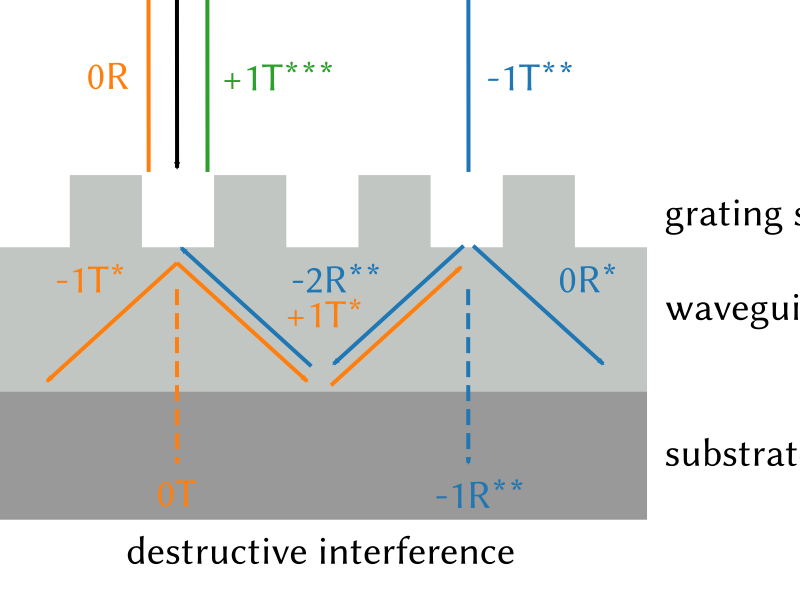
\includegraphics[width=\columnwidth]{graphics/generated/from-svg/30-waveguide-reflection.pdf}
  \caption{\label{fig:waveguide-reflection}Propagation of light within a waveguide mirror. The grating and waveguide layers have refractive index $n_H$, and sit atop a substrate of refractive index $n_L$. Blue arrows represent incident light and red arrows represent reflected light. In realisations of waveguide mirrors such as this, a thin etch-stop layer is placed between the grating and waveguide layers to assist fabrication \cite{Friedrich2011}.}
\end{figure}

Calculations by Heinert \etal{} \cite{Heinert2013} showed that a suitably optimised \gls{WGM} can provide a reduction in coating thermal noise amplitude of a factor of 10 at cryogenic temperature compared to the \gls{ETM} employed in Advanced LIGO at room temperature. Figure\,\ref{fig:coating-vs-grating-noise} shows Brownian thermal noise modelled for different numbers of bilayers (following \cite{Harry2002}) for the Advanced LIGO \gls{ETM}. As the dielectric mirror uses more bilayers to decrease transmissivity, the Brownian thermal noise contribution increases. The grating, however, requires only a change in grating parameters to produce a specific transmissivity, and this does not have a strong dependence on Brownian thermal noise.

\begin{figure}
  \centering
  \includegraphics[width=\columnwidth]{graphics/generated/from-python/30-coating-vs-grating-noise.pdf}
  \caption{\label{fig:coating-vs-grating-noise}Reproduction of the results from Heinert \etal{} \cite{Heinert2013} showing Brownian thermal noise in an Advanced LIGO style \gls{ETM} at room temperature versus that of a \gls{WGM} at cryogenic temperature, as a function of transmissivity. The markers in the coating curve represent the number of quarter-wavelength bilayers forming the dielectric stack. Each additional bilayer in the coating stack produces lower overall transmissivity, but also increases the Brownian thermal noise. The grating's Brownian thermal noise contribution is independent of transmissivity. The transmissivity of Advanced LIGO's ETM is shown as a vertical, dashed line.}
\end{figure}

Previous efforts to demonstrate grating structures as alternatives to dielectric mirrors have identified phase noise in the light reflected from the grating not otherwise present in dielectric mirrors \cite{Wise2005, Freise2007}. This effect arises from transverse motion of grating mirrors with respect to the incident light. Incident light at angle $\alpha$ is reflected into the m\textsuperscript{th} diffraction order, exiting at angle $\beta_m$ (see Figure\,\ref{fig:grating-propagation}). The change in path length $\delta l_L$ between the reflected and incident light is then
\begin{equation}
  \delta l_L = \zeta_a + \zeta_b = \delta y
  \left( \sin{\alpha} + \sin{\beta_m} \right),
\end{equation}
where $\zeta_a$ and $\zeta_b$ represent the relative optical path length of each depicted ray.
The phase modulation induced in the light reflected from the \gls{WGM} is proportional to Fourier frequency with a \SI{90}{\degree} phase lead over the transverse motion \cite{Barr2011}. The noise added to the reflected light can be enough to mitigate the improvement in coating thermal noise, as witnessed in a study of \nth{2} order Littrow gratings \cite{Barr2011}. Although \gls{WGM}s also possess gratings, the resonant waveguide structure has been shown in simulations by Brown \emph{et al.} to be invariant to transverse to longitudinal coupling \cite{Brown2013}.

\begin{figure}
  \centering
  \includegraphics[width=\columnwidth]{graphics/generated/from-svg/30-grating-propagation.pdf}
  \caption{\label{fig:grating-propagation}Optical path length changes $\zeta_a$ and $\zeta_b$ due to transverse motion of a Littrow grating. Incident light diffracted into a different order undergoes a path length change $\delta l_L = \zeta_a + \zeta_b$.}
\end{figure}

\begin{table}
  \centering
  \begin{tabular}{|l|l|}
    \hline
    \textbf{Parameter}    & \textbf{Value}            \\ \hline
    Materials             & \ce{SiO_2}, \ce{Ta_2O_5}, \\
                          & \ce{Al_2O_3}              \\ \hline
    Design $\lambda$      & \SI{1064}{\nano\meter}    \\ \hline
    Grating depth         & \SI{390}{\nano\meter}     \\ \hline
    Waveguide depth       & \SI{80}{\nano\meter}      \\ \hline
    Etch stop depth       & \SI{20}{\nano\meter}      \\ \hline
    Grating period        & \SI{688}{\nano\meter}     \\ \hline
    Fill factor           & 0.38                      \\ \hline
    Reflectivity          & 96\%                      \\ \hline
  \end{tabular}
  \caption{\label{tab:waveguide-parameters}Design parameters of the \gls{WGM} produced by Friedrich-Schiller Jena for the experiment to measure transverse to longitudinal coupling. It is similar to the one used in \cite{Friedrich2011}, with increased reflective surface area.}
\end{table}

There are two mechanisms by which grating mirrors can couple transverse motion into longitudinal phase changes (see Figure\,\ref{fig:waveguide-scanning}). The first is through transverse motion of the grating, which can in principle be minimised with appropriate suspension design. The second mechanism is the coupling of changes in the opposite cavity mirror's alignment into the spot position on the grating mirror. This effect is of particular importance to gravitational wave observatories, where longer arm lengths can increase its detrimental impact. For this reason the second mechanism is considered in more detail in this work.

In order to quantify its transverse coupling, a \gls{WGM} was produced in collaboration with Friedrich-Schiller University Jena, Germany (see Table \ref{tab:waveguide-parameters} for its properties). It was designed for light of wavelength \SI{1064}{\nano\meter}, and consisted of an etched grating structure on top of a waveguide layer, both tantala, on a silica substrate. This chapter details an experiment carried out to measure its transverse coupling level.

\begin{figure}
  \centering
  \includegraphics[width=\columnwidth]{graphics/generated/from-svg/30-waveguide-scanning.pdf}
  \caption{\label{fig:waveguide-scanning}Two ways in which light can be scanned across the surface of the \gls{WGM}. The left panel shows the effect of \gls{WGM} motion with respect to a static beam, while the right panel shows the effect of light beam motion (due to rotation of the cavity mirror opposite the \gls{WGM}) with respect to a static \gls{WGM}. The latter effect is the one primarily considered in this work.}
\end{figure}

\section{Experiment}

The fabricated \gls{WGM} was used as the input coupler for a \FP{} cavity, held on resonance using the Pound-Drever-Hall (PDH) technique \cite{Drever1983}. The error signal provided by the PDH technique represents changes in cavity length, and this can be fed back to the laser's frequency \emph{via} a frequency stabilisation servo.

\subsection{Cavity length signals}
\label{sec:lengthsignals}

A non-zero \gls{WGM} transverse to longitudinal coupling, $\omega_1$, produces a phase shift on the reflected light. This manifests itself as an effective change in cavity length, $\delta l_W$, as the laser light is scanned across its grooves by a rotation of the \gls{ETM}:
\begin{equation}
  \delta l_W \left( \theta, \kappa, \omega_1 \right) = \theta \kappa \omega_1,
  \label{eq:wgm-length-change}
\end{equation}
where $\theta$ is the \gls{ETM}'s rotation angle and $\kappa$ is the cavity's coefficient of \gls{ETM} rotation to transverse \gls{WGM} spot motion.

Additional cavity length changes are also produced \emph{via} two geometrical effects (see Figure\,\ref{fig:mirror-longitudinal-effect}). The first effect, $\delta l_s$, is due to the position of the beam with respect to the centre of the mirror's surface. For a rotation $\theta$, a beam offset from the centre of the mirror by a displacement $y$ will receive a change in (longitudinal) path length of
\begin{equation}
  \delta l_s \left( y, \theta \right) = y \tan{\theta} \approx y \theta
  \label{eq:offset-effect}
\end{equation}
for small angles. The second effect, $\delta l_d$, is due to the depth $d$ of the mirror, proportional to the rotation angle $\theta$. The position of the centre of the mirror with respect to the zero rotation case, $y_d$, is then
\begin{equation}
  y_d \left( d, \theta \right) = \frac{d}{2} \tan{\frac{\theta}{2}} \approx \frac{d}{4} \theta,
\end{equation}
and the change in path length this causes is
\begin{equation}
  \delta l_d \left( d, \theta \right) = y_d \tan{\theta} \approx \frac{d}{4} \theta^2.
\end{equation}
The total longitudinal effect $\delta l_E$ caused by the rotation of the \gls{ETM} is therefore
\begin{equation}
\delta l_E \left(y, \theta, d \right) = \delta l_s + \delta l_d \approx y \theta + \frac{d}{4} \theta^2.
\label{eq:etm-length-change}
\end{equation}

\begin{figure}
  \centering
  \includegraphics[width=\columnwidth]{graphics/generated/from-svg/30-mirror-longitudinal-effect.pdf}
  \caption{\label{fig:mirror-longitudinal-effect}Geometrical \gls{ETM} longitudinal effects. For a given rotation $\theta$ and spot centre position offset $y$, the (longitudinal) position change in the surface of the mirror (show in blue) as seen by the reflected light is approximately $y \theta + \frac{d}{4} \theta^2$. The straight, solid red line in the figure shows this longitudinal change.}
\end{figure}

Considering the \gls{ETM}'s level of rotation and its dimensions and mass, it is possible to calculate the cavity length change due to the two geometrical effects shown in Equation~\ref{eq:etm-length-change} and then, from the residual cavity length change, infer the \gls{WGM}'s coupling level. The phase effect associated with transverse to longitudinal coupling is expected to be independent of spot position, whereas there is a phase change about the \gls{ETM}'s centre of rotation. It is therefore expected that a spot position will exist, for a non-zero \gls{WGM} transverse coupling level, offset from the \gls{ETM}'s centre of rotation, for which there is a cavity error signal minimum. This effect arises as a result of $\delta l_W$ and $\delta l_{E}$ combining coherently (see Figure\,\ref{fig:coupling-contributions}). The spot position corresponding to the cavity error signal minimum allows the \gls{WGM}'s transverse to longitudinal coupling level to be inferred.

\begin{figure}
  \centering
  \includegraphics[width=\columnwidth]{graphics/generated/from-python/30-individual-factors.pdf}
  \caption{\label{fig:coupling-contributions}Simulations of indicative cavity longitudinal error signals during \gls{ETM} rotation for different levels of \gls{WGM} coupling. The signals are functions of the transverse position of the reflected light relative to the \gls{ETM}'s centre of rotation, the angle of rotation, the mirror depth and the \gls{WGM}'s coupling level. The rotation to longitudinal coupling of the \gls{ETM} (black dashed line) combines with the transverse to longitudinal coupling of the \gls{WGM} (red, green and blue dashed lines) to produce cavity length changes (red, green and blue solid lines). In this example configuration, the \gls{ETM} rotation is \SI{1e-7}{\radian}, the \gls{ETM}'s depth is \SI{0.1}{\meter} and the corresponding \gls{WGM} coupling levels are 1:370 (red), 1:3700 (green) and 1:37000 (blue).}
\end{figure}

Examples of \gls{WGM} coupling levels yielding cavity length changes smaller than (blue), larger than (red) and roughly equivalent to (green) the \gls{ETM}'s effects are shown in Figure\,\ref{fig:coupling-contributions}. For cases where the \gls{WGM}'s coupling level yields a significant cavity length change with respect to that of the \gls{ETM}'s rotation, coherent combination creates a trough offset from the \gls{ETM}'s centre of rotation.

% Coupling levels in fig:coupling-contributions
% rotation angle is 1e-7 rad (from plot_individual_factors script, an arbitrary choice, not the real level of rotation used in the experiment)
% rotation to sidemotion calibration from the experiment is 18.5119047619 metres / rad
%
% so sidemotion is 1851 nm
%
% red: longitudinal signal is 5e-9 m, so coupling is 1:370
% green: 5e-10 m, so 1:3702
% blue: 5e-11, so 1:37024

\subsection{The \GLASGOWTENM{}}
\label{sec:glasgow10m}

The \GLASGOWTENM{} facility provided a test bed in which the \gls{WGM}'s transverse to longitudinal coupling could be quantified. The prototype is housed in a Class 1000 clean room and consists of an input bench at atmospheric pressure and a vacuum envelope able to reach pressures of order \SI{e-3}{\pascal}. The envelope consists of nine \SI{1}{\meter} diameter steel tanks, each connected by steel tubes, arranged into two parallel arms of length \SI{10}{\meter}, with a shorter arm for input optics situated between them.

In the experiment, \SI{1064}{\nano\meter} laser light was passed through a single-mode fibre to provide spatial filtering and an electro-optic modulator (EOM) to impose RF sidebands on the light to facilitate PDH control. The light was then coupled into the vacuum system \emph{via} a periscope. This configuration can be viewed in Figure\,\ref{fig:prototype-setup}.

Tanks 2 and 3 housed a beam splitter and steering mirror, respectively, attached to double stage suspensions. In tanks 4 and 5 were sets of two triple suspension chains based on the GEO-600 design \cite{Plissi2000}. A viewport present to the rear of tank 5, and to the side of tank 1, allowed for light to exit the vacuum envelope for the purposes of sensing and control.

\begin{figure}
  \centering
  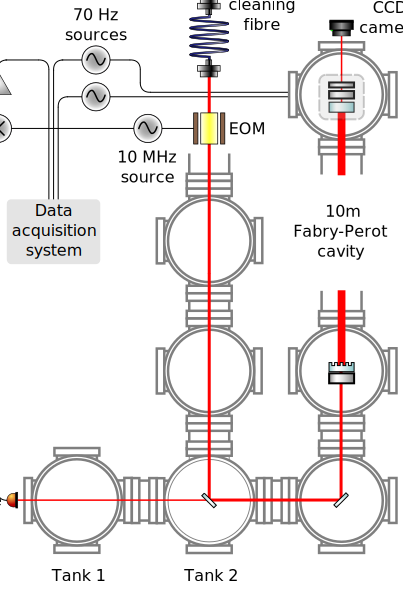
\includegraphics[width=\columnwidth]{graphics/generated/from-svg/30-waveguide-arm-in-prototype.pdf}
  \caption{\label{fig:prototype-setup}The experimental setup in the prototype facility. The laser light is passed through input optics (not shown), a mode cleaning fibre and an EOM before being coupled into the vacuum system \emph{via} a periscope. It then travels to tank 2 where it is reflected off a beam splitter and directed into one of the arms of the prototype by a steering mirror in tank 3. The two cavity mirrors in tanks 4 and 5 form a \FP{} cavity. The cavity mirrors are suspended from triple stage suspensions, and the beam splitter and steering mirror are both suspended from double suspensions. \\
  \\The \gls{ETM} is rotated in yaw using the \SI{70}{\hertz} source. It is fed to a coil driver where it is coupled into tank 5 \emph{via} a vacuum feedthrough. Coil formers on the front edges of the reaction mass contain wound copper wire connected to the vacuum feedthrough. Magnets are attached to the back of the \gls{ETM}. The reaction mass is behind the \gls{ETM}, containing a hole in its centre to allow light to exit the vacuum tank where it can be viewed with the CCD camera. A larger version of the contents of tank 5 can be viewed in the panel to the right of the figure. \\
  \\The cavity is held on resonance by the frequency stabilisation servo. This feeds back to the light's frequency \emph{via} the laser crystal's temperature below \SI{12}{\hertz} and its PZT above \SI{12}{\hertz} up to a unity gain frequency of \SI{14}{\kilo \hertz}.}
\end{figure}

The \gls{WGM} was attached to an aluminium block of mass \SI{2.7}{\kilo\gram} and suspended from tank 4's cascaded (triple) pendulum, forming the cavity's \gls{ITM}. A silica test mass, also \SI{2.7}{\kilo\gram}, with a \SI{40}{ppm} transmission coating, was used as the \gls{ETM}, suspended from a similar triple pendulum in tank 5. On the rear surface of the \gls{ETM} were three magnets for the purpose of actuation, the positions of which are shown in Figure\,\ref{fig:etm-rear}. With optimal alignment the mirrors formed an overcoupled cavity with finesse \num{155}.

\begin{figure}
  \centering
  \includegraphics[width=\columnwidth]{graphics/generated/from-svg/30-etm-rear.pdf}
  \caption{\label{fig:etm-rear}The positions of the magnets on the rear surface of the \gls{ETM}. The magnet designations used in this article are shown in red text. The top magnet is positioned at the centre of yaw, near the top of the mass. The left and right magnets are positioned \SI{56.3}{\milli\meter} either side of the centre of yaw. Coils on the \gls{ETM}'s reaction mass (not shown) are positioned coaxially behind each magnet.}
\end{figure}

A three-stage reaction chain was placed behind the triple pendulum of the \gls{ETM} to provide voice coil actuation upon the magnets on the \gls{ETM}'s rear surface. The upper and intermediate stages were identical to those of the chain carrying the \gls{ETM}, however\textemdash for the purposes of another experiment, not reported here\textemdash the lower stage was split into two parts separately suspended from the intermediate stage. The part closer to the \gls{ETM} was a \SI{1.8}{\kilo\gram} aluminium block that carried the voice coils. The other part was a \SI{0.9}{\kilo\gram} aluminium block required to balance the suspension.

\begin{table}
  \centering
  \begin{tabular}{|l|l|}
    \hline
    \textbf{Parameter}        & \textbf{Description}	      \\ \hline
    Cavity input power      & Approx. \SI{150}{\milli\watt}   \\ \hline
    \gls{ETM} transmissivity      & $40$~ppm                  \\ \hline
    \gls{ETM} radius of curvature & \SI{15}{\meter}           \\ \hline
    \gls{ETM} spot size           & \SI{2.138}{\milli \meter} \\ \hline
    \gls{ITM} transmissivity      & \SI{4}{\%}                \\ \hline
    \gls{ITM} radius of curvature & $\infty$                  \\ \hline
    \gls{ITM} spot size           & \SI{1.554}{\milli \meter} \\ \hline
    Cavity length           & \SI{9.81}{\meter}               \\ \hline
    Cavity finesse          & \SI{155}{}                      \\ \hline
    Cavity g-factor         & \SI{0.347}{}                    \\ \hline
    Beam waist size         & \SI{1.554}{\milli \meter}       \\ \hline
    Beam waist position     & At \gls{ITM}                    \\ \hline
    Sideband frequency      & \SI{10}{\mega\hertz}            \\ \hline
  \end{tabular}
  \caption{\label{tab:cavity-parameters}Cavity parameters.}
\end{table}

\subsection{Measuring cavity length changes}

An RF photodetector was placed at the viewport on tank 1, where it could view the light reflected from the cavity. By using PDH demodulation, the signal from this photodetector provided an error signal for the cavity length. This signal was fed back to the laser \emph{via} the frequency stabilisation servo to maintain cavity resonance. The frequency stabilisation servo's high frequency feedback signal\textemdash a voltage applied across the laser's piezoelectric transducer (PZT)\textemdash provided a means of calibrating cavity length changes at frequencies greater than \SI{12}{\hertz}. Using the PZT's frequency response, \SI{1.35}{\mega\hertz \per \volt_{rms}}, the cavity length change $\delta l$ per error signal volt could be calculated to be \SI{133}{\nano\meter \per \volt_{peak}}.

\subsubsection{The Pound-Drever-Hall technique}
\note{Describe PDH}

\subsubsection{Cavity control}
\note{Describe servos and filters used to lock the cavity}

\section{Measurements and analysis}
\label{sec:measurements}

From the orientation of the \gls{WGM}'s gratings, it was expected that actuation of the \gls{ETM} in yaw, which would scan the cavity light across the \gls{WGM}'s surface transverse to the direction of its grooves, would exhibit \gls{WGM} transverse to longitudinal coupling if present.

For the purposes of actuation upon the \gls{ETM}, two sinusoidal signals $V_L$ and $V_R$ (corresponding to the left and right voice coils on the \gls{ETM}'s reaction mass, respectively) were produced using separate, phase locked signal generators. A signal frequency of \SI{70}{\hertz} was chosen so as to be above the suspensions' pole frequencies but low enough to provide an adequate signal-to-noise ratio. The signals $V_L$ and $V_R$, with suitable balancing (see below), could then be actuated in- or out-of-phase to produce longitudinal or yaw actuation upon the \gls{ETM}, respectively.

When $V_L$ and $V_R$ were identical in magnitude but out-of-phase, the \gls{ETM}'s movement contained a linear combination of rotational and longitudinal components due to force imbalances between the voice coils. To ensure that actuation upon the \gls{ETM} contained only a yaw component, the cavity's longitudinal error signal was minimised during out-of-phase actuation by changing the gain of $V_L$. This balanced the magnitude of the torque applied by each actuator to the left and right sides of the \gls{ETM}. Any \gls{WGM} transverse to longitudinal coupling present would act with phase orthogonal to this voice coil actuation and would thus be unchanged by the torque balancing.

Pitch actuation upon the \gls{ETM}, which would scan the cavity light in a direction parallel to the \gls{WGM}'s grooves, was not expected to contribute to the cavity's error signal via the \gls{WGM}'s coupling. However, unintended pitch actuation upon the \gls{ETM} would couple into the cavity's length \emph{via} the same geometrical mechanism as yaw shown in Equation~\ref{eq:etm-length-change}. To minimise the \gls{ETM}'s pitch component during actuation in yaw, the cavity's error signal was minimised by applying an offset voltage to the top coil. In practice, minimal pitch coupling was achieved when the offset signal was zero.

\subsection{Actuator calibration}

To calibrate the cavity's longitudinal response to voice coil actuation, the voice coils were actuated with the balanced $V_L$ and $V_R$ signals in-phase at a frequency $f = \SI{70}{\hertz}$ for a period of \SI{120}{\second}. This, along with the \gls{ETM}'s mass $m$, could then be used to obtain the force applied to the \gls{ETM} by the voice coils:
\begin{equation}
  F = 4 \pi^2 f^2 m \delta l.
  \label{eq:force-calibration}
\end{equation}

\subsection{Measurement of waveguide mirror transverse to longitudinal coupling}
\label{sec:length-changes}

% The spot positions were scaled to account for the defocusing effect - see https://arran.physics.gla.ac.uk/labbooks/index.php?LabBook=JIF_Diff, "Working out Monitor Perspective", October 29th 2013

Four spot positions corresponding to $y$ in Equation~\ref{eq:offset-effect} were chosen across the surface of the \gls{ETM}. The input beam was aligned to the cavity axis corresponding to each spot position using the beam splitter and steering mirror nearest to the \gls{ITM}, and the cavity mirrors were aligned to create a fundamental mode resonance. The voice coil signals $V_L$ and $V_R$ were set out-of-phase to produce motion on the \gls{ETM} in yaw. The magnitudes of $V_L$ and $V_R$ were not altered between the longitudinal calibration and this yaw actuation, so it was expected that the previously outlined minimisation of yaw to tilt actuation would also result in minimal longitudinal to tilt actuation. The cavity length signal was recorded for a period of \SI{300}{\second}.

For each nominal spot position an additional measurement was taken with $V_L$ set to $\pm \SI{0.1}{\volt}$ from its balanced setting for a period of \SI{60}{\second}. This allowed two additional data points to be obtained for each spot position. By calculating the gradient (cavity length change per spot position with respect to the centre of yaw) of the central and inner-left spot positions, it was possible to assign an effective spot position for each of the offset points.

The spot positions used to obtain cavity error signals are shown in Table~\ref{tab:spot-positions}. These positions are shown with respect to the centre of the \gls{ETM}'s reflective surface. The spot positions were subject to two sources of error: the measurement of the spot positions with respect to the centre, and the error in the \gls{ETM}'s centre of rotation due to misalignment between the voice coils and their corresponding magnets. The spot position error was assumed to be \SI{\pm1}{\milli\meter} from visual inspection of the suspensions, measured \emph{via} the CCD camera placed in transmission of the \gls{ETM}, using the known width of the \gls{ETM}'s reaction mass as a calibration.

Misalignment between the voice coils and magnets can lead to unintended torque and longitudinal actuation, confusing the calibration. To evaluate whether this effect could be significant, a small experiment was configured as shown in Figure\,\ref{fig:misaligned-voice-coil-experiment}. A rod was placed above a magnet with the voice coil attached to its end, with both magnet and voice coil having the same dimensions as those of the main experiment. The magnet was glued to a thick perspex disc attached to the base edge of an upturned plastic cup to allow the force applied to the magnet to rigidly couple to the base of the cup. The cup was itself placed upon scales accurate to \SI{1}{\micro\gram} and a translation stage with \SI{25}{\micro\meter} precision.

\begin{figure}
  \centering
  \includegraphics[width=\columnwidth]{graphics/generated/from-svg/30-magnet-offset-experiment.pdf}
  \caption{\label{fig:misaligned-voice-coil-experiment}Experiment to measure the effect of misaligned voice coil actuation.}
\end{figure}

With the front edge of the voice coil separated from the base of the magnet by \SI{7.9}{\milli\meter}\textemdash close to that of the main experiment\textemdash a series of force measurements were taken. A constant current source of \SI{50}{\milli\ampere} was applied through the coil while incrementing the translation stage in steps of \SI{0.1}{\milli\meter}. The results in Figure\,\ref{fig:misaligned-voice-coil-results} show that the effect is negligible within the main experiment's alignment error, with an upper limit for the drop in force determined to be \SI{0.11}{}\% given the error from determining the alignment by visual inspection. This corresponds to a negligible error of less than \SI{\pm30}{\micro\meter} in the results, which is dominated by the spot position error.

\note{Add coil sweet spot plot?}

\begin{figure}
  \centering
  \includegraphics[width=\columnwidth]{graphics/generated/from-python/30-magnet-offset.pdf}
  \caption{\label{fig:misaligned-voice-coil-results}Change in force as a function of transverse displacement from voice coil axis. A quadratic fit has been applied to the data and the axes shown are with respect to the position and magnitude of the maximum fitted force, following the assumption that this position is nearest to the optimal alignment. This fit is probably a worst case scenario, as the magnet was positioned close to the voice coil's position of maximum force, where the field gradient is quite flat. \checkme{Assuming the voice coils and magnets were aligned within \SI{0.5}{\milli\meter}, the maximum drop in force would have been negligible\textemdash less than 1\%\textemdash and so this explanation can be ruled out.}}
\end{figure}

\begin{table}
  \centering
  \begin{tabular}{|c|c|c|}
    \hline
    \multicolumn{3}{|c|}{\textbf{Spot position [\SI{}{\milli \meter}]}} \\ \hline
    \SI{-0.1}{\volt} & \SI{0.0}{\volt} & \SI{+0.1}{\volt}               \\ \hline\hline
    \num{-12.9} & \num{-12.5} & \num{-12.1}                             \\ \hline
    \num{-5.4} & \num{-5.0} & \num{-4.6}                                \\ \hline
    \num{-0.4} & \num{0.0} & \num{0.4}                                  \\ \hline
    \num{12.1} & \num{12.5} & \num{12.9}                                \\ \hline
  \end{tabular}
  \caption{\label{tab:spot-positions}Spot positions on the \gls{ETM} for the far left, inner left, central and right positions, respectively. The positions are shown in groups of three corresponding to the offset applied to $V_L$. All spot positions have an error of \SI{\pm1}{\milli\meter}.}
\end{table}

Knowledge of the distance of the \gls{ETM}'s voice coils from the centre of rotation, $y_c$; the \gls{ETM}'s moment of inertia, $I$; the coil driving frequency, $f$; and the force calibration from Equation~\ref{eq:force-calibration}, allowed the rotation angle to be obtained geometrically using the relation
\begin{equation}
  \theta = \frac{F y_c}{4 \pi^2 f^2 I}.
  \label{eq:rotation-calibration}
\end{equation}
The numerical simulation tool \emph{FINESSE} \cite{Freise2004} was then used to calculate $\kappa$ for the cavity parameters shown in Table~\ref{tab:cavity-parameters}. This was determined to be \SI{18.5}{\meter \per \radian}. The \gls{WGM}'s transverse displacement was then the product of $\kappa$ and $\theta$.

\subsection{Analysis of the coupling level}
\label{sec:simulations}
Using the known contribution to the cavity length signal from the rotation of the \gls{ETM}, $\delta l_E$, and the cavity length signals $\delta l$ measured during the experiment, the \gls{WGM}'s coupling level could be calculated statistically using Bayes' theorem. For this experiment, Bayes' theorem can be expressed mathematically as:
\begin{equation}
  p \left( \vec{\omega} | \mathcal{D} \right) \propto p \left( \mathcal{D} | \vec{\omega} \right) p \left( \vec{\omega} \right),
  \label{eq:bayes}
\end{equation}
where $p \left( \vec{\omega} | \mathcal{D} \right)$ is the probability density distribution of the experimental parameters, $\vec{\omega}$, given the observed data, $\mathcal{D}$ (the \emph{posterior}); $p \left( \mathcal{D} | \vec{\omega} \right)$ is the likelihood and $p \left( \vec{\omega} \right)$ is the probability distribution of the experimental parameters. The observed data $\mathcal{D}$ are the measured cavity error signals for each of the spot positions.

In this analysis we are primarily interested in estimates of the model parameters. We are therefore free to ignore the constant evidence factor $p \left( \mathcal{D} \right)$ present in Bayes' theorem when calculating the posterior. In the future it may be of interest to compare different models for the coupling level (or lack thereof), in which case the evidence could be calculated to obtain a model odds ratio.

\subsubsection{Model and parameters}
To obtain a posterior for the \gls{WGM}'s coupling level, it was necessary to build a model and state prior belief of the parameters' probability distributions.

In the model, the \gls{ETM}'s geometrical longitudinal effect at arbitrary spot position $y$ (Equation~\ref{eq:etm-length-change}) for the rotation and mirror depth used in the experiment was combined coherently with a specified level of \gls{WGM} transverse to longitudinal coupling, $\omega_1$. It was then possible to predict the total change in cavity length $\delta l$ as a function of spot position $y$, given the fixed parameters $\theta$, $\kappa$ and $d$, using equations~\ref{eq:wgm-length-change} and \ref{eq:etm-length-change}:
\begin{equation}
  \begin{split}
    \delta l \left( \vec{\omega}, y, \theta, \kappa, d \right) & = \delta l_W \left( \theta, \kappa, \omega_1 \right) + \delta l_E \left( y, \theta, d \right) \\
    & \approx \theta \kappa \omega_1 + y \theta + \frac{d}{4} \theta^2.
  \end{split}
\end{equation}

The effect of \emph{beam smearing} was also considered. The suspended optics contain residual displacement noise, leading to a broadening of the trough at which the \gls{ETM}'s longitudinal coupling and any \gls{WGM} coupling cancel (see Figure\,\ref{fig:coupling-contributions}). To model this effect, the assumption was made that the motion of the spots on the \gls{ETM} followed a Gaussian distribution about their nominally measured position. Eight-hundred small `offset distances' $\delta y$ were applied uniformly to the spot positions, drawn from a randomly generated Gaussian distribution. The number of offset distances was chosen as a compromise between adequate statistical significance and technical constraints. Calculating the cavity length change as a function of spot position for each of these offset positions, and combining them in an uncorrelated sum, allowed an average, `smeared' signal to be modelled which more closely resembled the measurements. The standard deviation of the Gaussian distribution was an additional parameter, $\omega_2$, provided as an input to the model.

The summing of signals introduced by the modelling of beam smearing led to an artificial increase in the magnitude of the model's predicted cavity length signals. To compensate for this effect, a further parameter was introduced: a multiplicative scaling factor, $\omega_3$, applied uniformly to the model. This factor also had the additional effect of compensating for the uncertainty in the calibrated cavity length signals. By marginalising over a suitable distribution of scaling factors, it was possible to account for this uncertainty in the analysis of the \gls{WGM}'s coupling level. The model used in the analysis to predict the smeared, scaled cavity length change, $\delta l'$, was then:
\begin{equation}
  \delta l' \left( \vec{\omega}, y, \theta, \kappa, d \right) = \omega_3 \sqrt{\sum_{i=1}^{800} \delta l \left( \vec{\omega}, y + \delta y_i, \theta, \kappa, d \right)^2},
  \label{eq:model}
\end{equation}
where $\delta y_i$ is the $i^\text{th}$ offset distance, drawn from a Gaussian distribution with standard deviation $\omega_2$.

\subsubsection{Likelihood}
The likelihood function assumed for the model was a Gaussian distribution,
\begin{equation}
  p \left( \vec{\omega} | \mathcal{D} \right) \propto \exp \left( -\frac{1}{2} \sum_{i=1}^{N} \frac{\left( \mathcal{D}_i - \delta l' \left( \vec{\omega}, y_i, \theta, \kappa, d \right) \right)^2}{\sigma^2} \right),
  \label{eq:likelihood}
\end{equation}
where $N$ is the number of spot positions and $\sigma^2$ is the (identical) variance of each of the measured spot positions.

\subsubsection{Priors}
Bayes' theorem requires an assumption of probability distributions (\emph{priors}) for each of the free parameters prior to the consideration of the measured data. The assumptions made for each free parameter in the model can be found in Table~\ref{tab:priors}. The upper bound on coupling was assumed to be a factor \num{10} better than the grating mirror measured in~\cite{Barr2011}, given the indication from~\cite{Brown2013} that no coupling is present. The bounds on the scaling factor and spot smearing standard deviation were chosen from earlier observations of the behaviour of the signals during the experiment. All priors were assumed to be uniform.

\begin{table}
  \centering
  \begin{tabular}{|p{3cm}|c|c|c|}
    \hline
    \textbf{Parameter}   & \textbf{Symbol}     & \textbf{Distribution} & \textbf{Dimensions} \\ \hline
    \gls{WGM} transverse to longitudinal coupling & $\omega_1$ & Uniform, $\left[ 0, \frac{1}{1000} \right]$ & $\frac{\SI{}{\meter} \text{ (longitudinal)}}{\SI{}{\meter} \text{ (transverse)}}$ \\ \hline
    Spot smearing noise standard deviation & $\omega_2$ & Uniform, $\left[ 0, 3 \times 10^{-3} \right]$ & $\SI{}{\meter} \text{ (transverse)}$ \\ \hline
    Calibration scaling                    & $\omega_3$ & Uniform, $\left[ 0, \frac{1}{10} \right]$ &  \\ \hline
  \end{tabular}
  \caption{\label{tab:priors}The distributions assumed for each of the free parameters in the model, along with their dimensions, prior to the computation of the posterior.}
\end{table}

\subsubsection{Algorithm}
A form\footnote{\emph{``Yet Another Matlab MCMC code''} by Matthew Pitkin. Available as of time of writing at \url{https://github.com/mattpitkin/yamm}.} of the Metropolis-Hastings Markov-Chain Monte-Carlo (MCMC) algorithm \cite{Hastings1970} was applied to the model to marginalise over the three parameters. The outputs of the MCMC are a chain of samples (values at each parameter) that are drawn from the posterior distribution. A histogram of samples for a given parameter gives the marginal posterior distribution for that parameter from which the mean and standard deviation can be calculated.

To ensure the convergence of the MCMC on the posterior, a `burn-in' period of \num{100000} iterations was performed. The convergence was verified manually following completion. A further \num{100000} iterations were then used to sample from the posterior and this second set is the one that we used for our results.

\section{Results}
\label{sec:summary}
From the parameter marginalisation it was possible to produce a posterior probability density distribution for the coupling level as shown in Figure\,\ref{fig:wgm-coupling-prob}. The coupling level predicted from the distribution is bounded between 0 and 1:17000 with 95\% confidence, with a mean coupling level of 1:27600. The probability density distributions for the scaling and standard deviation parameters are shown in Figures\,\ref{fig:posterior-scaling} and \ref{fig:posterior-stddev}, respectively. The scaling posterior distribution indicates a mean value of \num{29.3e-3} with standard deviation \num{0.94e-3}. The posterior distribution for the beam smearing parameter indicates a range of possible values between \num{0} and \SI{1.3e-3}{\meter}. All of the posterior distributions lie well within their prior ranges (see Table\,\ref{tab:priors}).

The measured cavity length signals as well as the 95\% upper limit and mean \gls{WGM} coupling level predicted by the analysis are shown in Figure\,\ref{fig:wgm-coupling}. The phase discrepancy between the model and the measurements, as witnessed in this figure most profoundly for the spot positions around \SI{-5e-3}{\meter}, is thought to be an artefact from the modelling of the beam smearing effect. The residual test mass motion that motivated the inclusion in the model of beam smearing may have contained some non-Gaussian behaviour.

The upper limit on the predicted coupling level, 1:17000, represents a significant improvement over previously measured grating designs such as the \nth{2} order Littrow grating measured in \cite{Barr2011}, where the coupling factor was of order 1:100.

\begin{figure}
  \centering
  \includegraphics[width=\columnwidth]{graphics/generated/from-python/30-posterior-coupling.pdf}
  \caption{\label{fig:wgm-coupling-prob}Posterior probability density distribution of \gls{WGM} coupling levels (in units of meters longitudinal per metre transverse) yielded by statistical analysis of the data. The shaded region shows the coupling levels falling within the most probable 95\% of the distribution.}
\end{figure}

\begin{figure}
  \centering
  \includegraphics[width=\columnwidth]{graphics/generated/from-python/30-posterior-scaling.pdf}
  \caption{\label{fig:posterior-scaling}Posterior probability density distribution of scaling applied to the model's predicted longitudinal signal.}
\end{figure}

\begin{figure}
  \includegraphics[width=\columnwidth]{graphics/generated/from-python/30-posterior-stddev.pdf}
  \caption{\label{fig:posterior-stddev}Posterior probability density distribution of the standard deviation assumed for the Gaussian distribution used to model beam smearing.}
\end{figure}

\begin{figure}[H]
  \centering
  \includegraphics[width=\columnwidth]{graphics/generated/from-python/30-coupling-best-fit.pdf}
  \caption{\label{fig:wgm-coupling}Measurements and simulations of the cavity length signal for spot positions with respect to the \gls{ETM}'s centre of yaw. The calibrated cavity length change per radian (vertical axis) from the measurements is shown (blue stars) alongside the model's simulated cavity length changes per radian for the mean (red), 95\% upper limit (green) and zero (black) \gls{WGM} coupling levels. The simulated plots use a scaling factor of \num{29.3e-3} and a beam smearing standard deviation of \SI{0.8e-3}{\meter}.
  \bigskip
  \\ Error bars are shown on the measured spot positions corresponding to their uncertainty. The errors in cavity length change are obtained from the noise floor surrounding each measurement. The noise floors were approximately constant for all measurements, with mean value \SI{8e-5}{\meter \per \radian}. Phase error bars are visible for the central values. The errors on each phase measurement, from left to right, are: \num{+-0.0188}, \num{+-0.0254}, \num{+-0.0283}, \num{+-0.1387}, \num{+-0.1721}, \num{+-0.2178}, \num{+-3.2726}, \num{+-3.2303}, \num{+-2.0603}, \num{+-0.0385}, \num{+-0.0342} and \num{+-0.0336} degrees.}
\end{figure}

\section{Outlook}
The evidence for transverse to longitudinal coupling is consistent with zero from Figure\,\ref{fig:wgm-coupling-prob}, though it is not the most likely value from the experiment despite the literature suggesting otherwise. A future improvement upon this experiment might be to perform local measurements of the rotation of the \gls{ETM} with multiple sensors, to avoid the calibration susceptible to measurement error outlined in Section\,\ref{sec:length-changes}.

While the reduction in Brownian thermal noise in \gls{WGM}s is a clear advantage to future gravitational wave detectors, other technologies at similarly early stages of technical readiness present similar improvements, such as the use of crystalline coatings. The mirror coating technique that eventually becomes standard may depend on the direction that another field, fabrication engineering, takes in the near future.